
\begin{figure*}
 \centering 
    \begin{subfigure}[t]{1.45in}
        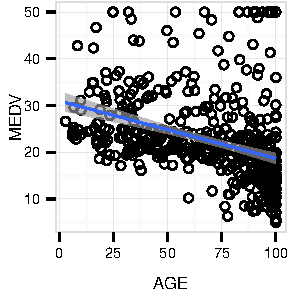
\includegraphics[width=1.45in]{images/AGE-MEDV.pdf}
        \caption{Input scatterplot}
        \label{fig:method_original}
    \end{subfigure}
    \begin{subfigure}[t]{1.5in}
  	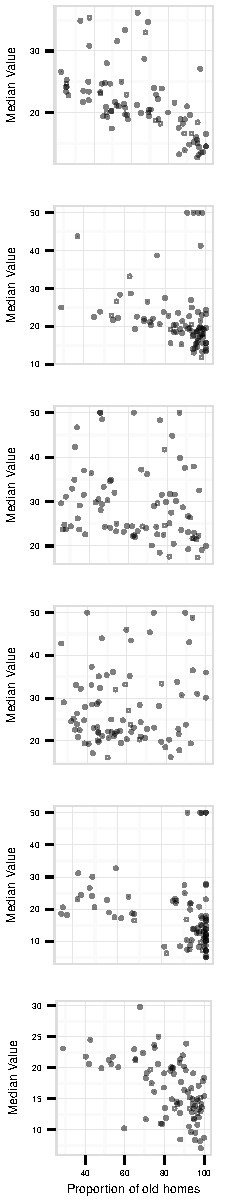
\includegraphics[width=1.5in]{images/DIS.pdf}
	\caption{Partitioned by distance to an employment center}
	 \label{fig:method_actual}
    \end{subfigure}
    \begin{subfigure}[t]{1.5in}
 	 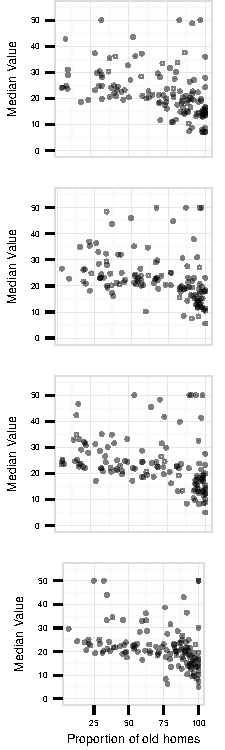
\includegraphics[width=1.5in]{images/randCluster.pdf}
     \vspace{-0.37cm}
 	 \caption{Partitioned by random permutation}
	 \label{fig:method_random}
    \end{subfigure}
     \begin{subfigure}[t]{2.5in}
 	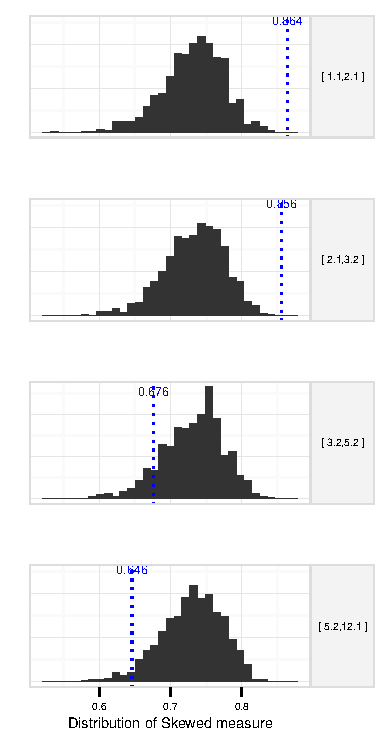
\includegraphics[width=2.5in]{images/hist-DIS.pdf}
	\caption{Distribution of skewness}
	 \label{fig:method_dist}
     \end{subfigure}
   \caption{Illustration of our method of evaluating small multiple displays. (a) The input scatterplot of interest. (b) Partitions determined by the mean distance to Boston's five employment centers. (c) Randomly permuted partitions of data. (d) Distribution of Skewed scagnostics for the randomly permuted partitions. The overlaid blue lines are the corresponding true scores of the partitions in (b). The blue lines are outliers, indicating that they likely did not arise due to chance. Our algorithm will score the small multiple display in (b) highly.}
\end{figure*}


\section{Method}
\label{sec:method}

In this section we propose a new method for automatically selecting good small multiple displays. Our approach takes three inputs from the analyst:
\begin{enumerate}
\item a scatterplot which the user wants to partition into a small multiple display,
\item a scagnostic that measures the presence or absence of a visual pattern of interest to the user, and
\item a list of potential partitioning variables.
\end{enumerate}
The output is a scoring of the small multiple displays produced by each partitioning variable.

In the following section, we describe desirable properties for small multiple displays that we use to motivate our approach. The next section describes our method in the context of a running example.

\subsection{Goodness-of-Split Criteria}
To guide our approach, we formulated the following four goodness criteria. Partitioning variables should be chosen such that the resulting small multiple displays are:
\begin{itemize}
\item \emph{Visually rich}: We want small multiple displays that convey rich visual patterns, as captured by the cognostic provided by the analyst. In contrast to statistical methods, such as ANOVA, which are based on relatively simple summary metrics with closed-form distributions, most cognostics involve complicated processing and do not follow a known distribution.

\item \emph{Informative}: The purpose of a small multiple display is to help explain patterns in the input visualization. We want to prefer partitioning variables that add information to the display, supporting the user in their analysis. Partitions that randomly split the data are not useful since they do not contain any more information than the original plot.

\item \emph{Well-supported}: For some data sets, particularly those with outliers or with a small number of data points, strong visual patterns can occur by chance. These spurious patterns are misleading; they appear informative, but are not. We would like to detect and downweight such  patterns, guiding analysts to more robust results.

\item \emph{Parsimonious}: A small multiple display with many partitions can be very difficult to read and understand. All things being equal, we want to favor splitting into as few plots as possible, while still providing an informative display.
\end{itemize}

\subsection{Algorithm}

Our approach is based on a simple intuition: effective small multiple displays are those whose component plots have cognostic scores that are very unlikely to have arisen due to chance. In this section, we describe a method for evaluating this likelihood using a \emph{randomized permutation test}, which is a non-parametric statistical significance test.

Our algorithm works by considering each potential partitioning variable individually. For each partitioning variable, we evaluate the cognostic measure on each component plot in the resulting small multiple, resulting in a vector of \emph{true} scores. We then repeatedly randomly permute the values of the partitioning variable, assigning each data point to a random partition, and reevaluate the cognostic score for each component plot. These randomized cognostic scores give us a vector of \emph{simulated null distributions}, capturing how likely different cognostic scores are to arise just by chance for each component plot.

We then compare the true scores to the null distributions by evaluating a z-score. This gives us a normalized measure that indicates how far visual pattern in the true partition is from a random partition. The z-score for each component plot $i$ of the small multiple display is:
$$z_i = \frac{(X_i-\mu_i)}{\sigma_i}$$ 
where $X_i$ is the true cognostic value of the $i$-th partition and $\mu_i$ and $\sigma_i$ are the mean and standard deviation of the cognostic measures over the repeated random permutations of the $i$-th partition. We use a z-score, rather than an order statistic because it is common for the true value to fall well outside the range of the simulated null distribution.

Finally, to get a score for the whole small multiple display, we use the maximum absolute z-score across all the component plots: 
$$z = \max_{i=1}^k |z_i|$$
Using the maximum results in high scores for small multiple displays that have strong, interesting patterns in at least one component plot. This worked well in our experimentation. However, it may discount small multiple displays with weaker patterns in many or all the component plots. This is discussed more in Section~\ref{sec:discussion}. 

To demonstrate how this algorithm works, consider the example in Figure~\ref{fig:method_original} showing the relationship between the median value of owner-occupied homes (in thousands of US dollars) and the proportion of owner-occupied units built prior to 1940. This dataset contains information collected by the U.S Census Service concerning housing in the area of Boston, Massachusetts~\cite{Harrison1978}. We see that as the proportion of older houses increases, the median value decreases. However, the distribution is skewed and an analyst may wonder if there is another variable that might reveal more about this relationship.
To do so, they can run our algorithm using Wilkinson et al.'s \emph{skewness} scagnostic.

Our algorithm will iterate through the possible partitioning variables scoring each one. Figure~\ref{fig:method_actual} shows the small multiple display resulting from partitioning on the binned distance to an employment center, one of the variables in the data set. Notice that, in contrast to the original plot, the density of the top two plots (representing a shorter distance to an employment center) appears substantially shifted to the right. While the bottom two plots (longer distances to an employment center) are shifted to the left. These differences will result in skewness scores that are substantially different from the original plot. 

However, it is possible that these shifts may have arisen due to random chance. Thus, our algorithm randomly permutes the values of the partitioning variable, producing the small multiple display in Figure~\ref{fig:method_random}. These plots show no sign of the change in skewness and look similar to the original plot. 
Our algorithm does this repeatedly, producing a distribution of possible random skewness values. The result of this process is shown in Figure~\ref{fig:method_dist}. The black histograms show the distribution of the skewness scagnostic for the random permutations. The blue lines show the skewness scagnostic for the actual variable---the distance to employment center. For the top two plots, the blue line is to the right of the histogram, indicating that the skewness of these two plots is much higher than we would expect to occur by chance. The bottom two have lower skewness than we would expect by chance, but the values are inside the simulated distribution, so there's less evidence for them.

After computing z-scores for these four distributions, we use the maximum absolute z-score as the overall score for this small multiple display. This partitioning variable, distance to employment center, is the highest rated in this data set and would be recommended to the analyst. The small multiple display offers a visual explanation of the relationship between employment center locations to the neighborhoods in Boston---areas with older, lower-valued homes are close to employment centers while newer, higher-valued homes tend to be further away from employment centers. The analyst can see the details of that correlation in the partitions of the display.
